\documentclass[a4paper, 11pt, titlepage]{article}
%\usepackage{color}
%\definecolor{light-gray}{gray}{0.95}

\usepackage{xcolor}
\usepackage{alltt}
\usepackage{url}
\usepackage{tikz}
\usepackage{ulem}
\usepackage{setspace}
\usetikzlibrary{trees}

% Command for inserting a todo item
%http://midtiby.blogspot.ie/2007/09/todo-notes-in-latex.html
\newcommand{\todo}[1]{%
% Add to todo list
\addcontentsline{tdo}{todo}{\protect{#1}}%
%
\begin{tikzpicture}[remember picture, baseline=-0.75ex]%
\node [coordinate] (inText) {};
\end{tikzpicture}%
%
% Make the margin par
\marginpar{%
\begin{tikzpicture}[remember picture]%
\definecolor{orange}{rgb}{1,0.5,0}
\draw node[draw=black, fill=orange, text width = 3cm] (inNote)
{#1};%
\end{tikzpicture}%
}%
%
\begin{tikzpicture}[remember picture, overlay]%
\draw[draw = orange, thick]
([yshift=-0.2cm] inText)
-| ([xshift=-0.2cm] inNote.west)
-| (inNote.west);
\end{tikzpicture}%
%
}%

\definecolor{light-gray}{gray}{0.95}
% Compensate for fbox sep:
\newcommand\Hi[2][light-gray]{%
  \hspace*{-\fboxsep}%
  \colorbox{#1}{#2}%
  \hspace*{-\fboxsep}%
}

\title{Technical Report}

\begin{document}
\onehalfspacing
\maketitle

\tableofcontents

\todo{Titles are subject too (and probably should in a lot of cases) change}

\section{Introduction}

\subsection{Motivation}
What is the internship; motivation and description

As part of my undergraduate studies I have elected to participate in the internship program run by the School of Computer Science and Statistics in Trinity College Dublin. The main motivation for this is the personal belief that education is made meaningful by application , that the context of a professional working environment would help to cement the knowledge gained in university. It should also draw attention to area of weakness that need to be improved upon.
Additionally, a professional working environment has a substantially different focus to that of a university. While both depend on the individual to self educate to achieve a certain goal, the motivation for this, how they go about it, and what goals are set differ substantially. My hope was that an internship would remove the play-pen walls and make me accountable for what I achieved or failed to achieve. University has a focus on collaboration, but in the majority of cases assessment is carried out on and individual basis. When working on a team, an individuals efforts directly impact the work done by others and as such there is greater accountability for ones actions. I have experienced all of this during a previous, shorter internship and seen the benefit in my attitude towards work and study as well as my overall personal development.

Description here

\todo{Rewrite that awful paragraph above} 

\subsection{Goals}

Upon arriving at Mastercard I was introduced to some of the team and my mentor, Peter Groarke. We immediately set to work and a brief road map was laid out. No formal goals were decided but Peter and the others walked me through a series of steps:
\begin{itemize}
\item Set up a working development environment.
\item Become familiar with software development life cycle at Mastercard and supporting infrastructure.
\item Contribute functioning code.
\end{itemize}
The main objective was to put me to work as soon as possible. This was my own personal objective and, happily, seemed to be inline with the objective of my mentor. As far as I am aware, there was no overall plan for the entire internship at the beginning. An assessment of my skill level was needed before that could be considered.

The first task assigned to me was to interface SMART with Cronos. SMART, Something Mastercard Authorization Rules Tool \todo{Get acronym} is an inhouse system testing tool used to send mock requests to the Retail API server. Cronos is another server used for retrieving certain system information. My own personal goal was to learn new and interesting programming concepts and technologies. \todo{Loads more detail}

\subsection{Approach (State of the art)}
Slightly reflective, what was my approach to the internship. Set goals with mentor, spent time learning system, learning new skills, development. Repeat steps 2 to 4. In reality is more development and learn as I go.

As stated, my initial goal was to start contributing as quickly as possible. This meant checking working code into subversion. The first step was to setup a working development environment. 
The majority of the first week was spent trying to install and configure a working GNU/Linux environment. The vast majority of the development work done in InControl targets Unix platforms. Linux is also my personal preference of operating system. The InControl department maintains a script used to automatically configure a new development environment. The idea was to simply setup a working Linux install and run the script. The first distribution I tried was one I had used for years. However, the updated version was considerably unstable when I attempted to deploy it. It took three days for me to identify the problem as the distribution, not the inhouse environment setup script. I switched distribution and had a working environment within hours. The next step was to become somewhat familiar with the InControl Platform. This consisted of reading any documentation I could get my hands on, experimenting with the system itself and looking through the system database, the core of the InControl platform.
InControl have a substantial but somewhat poorly indexed wiki which become my main source of documentation, other than the developers. Aside from the InControl platform I also tried to understand how credit card transactions were routed and processed. This was necessary to give the InControl platform context.
A large portion of my first few weeks was spent learning how 

\subsection{Overview of contents}


\section{Internship in Context}
SDL goes here. Derive requirements of testing from literature; blackbox functionality testing. Derive rest of requirements from actual company requirements. Describe existing system, enough detail to give context.

Orbiscom Ireland, acquired by Mastercard in 2009, develop a product called InControl. The acquisition allowed Mastercard to incorporate InControl into their Value Added Services, a range of products that tie in closely with their core business, the processing of electronic payments. Until 2010 Mastercard Ireland was still primarily concerned with the development of InControl. A division of Mastercard Labs was setup within Mastercard Ireland in 2011. As Mastercard continues to grow, more and more departments are being given a presence within Ireland. This report documents the activities and projects undertaken while working for InControl. Since their acquisition Orbiscom have become completely integrated into Mastercard and have ceased operating as Orbiscom entirely. InControl has been split into two different products. InControl Direct exists to support Orbiscoms original customers as is managed and maintained entirely within the InControl department. The second product, InControl is an adapted version of the original product. Where InControl Direct is deployed to and hosted by banks, InControl is hosted on BankNet, Mastercards global payments network. In order to explain the services offered by the InControl platform, it is useful to explain how the credit card payment process works.

InControl and Orbiscom are used somewhat interchangeably in the rest of the document. Orbiscom is a keyword used throughout the code base. All of the packages still begin with \textit{com.orbiscom}

\subsection{The Four Party Model}
The credit card payment scheme employed by Mastercard involves four separate parties, for this reason it is referred to as the four party model. There are alternate models in use, but Mastercard employs the four party model as it allows the issuing of payment cards to be handled by separate financial institutions. This leaves less overhead for Mastercard and also insures interoperability between the various financial institutions. The credit card holder typically initiates the payment and is represented by a credit card issuing bank, or an issuer. The merchant involved in the payment is represented by an acquiring bank, or an acquirer. Each successful payment goes through three stages; Authorization, Clearing and Settlement.
\subsubsection{Authorization} The card-holder submits their payment card details to the merchant. The merchants bank, the acquirer, sends a request to Mastercard to identify the card-holders issuing bank. Once this has been determined and the card has been verified the payment is forwarded, by Mastercard, to the issuing bank. It is worth noting that this is the stage in the process where the InControl service is applied if needed. The card-holders bank approves the purchase and blocks the funds in the card-holders account. No money has been transfered from the card-holders account, the money has merely become unusable by the card-holder. The issuing bank forwards the approval to Mastercard, who forwards it to the acquirer who in turn forwards it to the merchant. The payment has now been approved. 
\subsubsection{Clearing} Sometime after the payment has been authorized, usually at the end of the week, the merchant submits all of their authorized payments to clearing. This is a batch process that occurs at certain set times. After a payment has been cleared the funds have effectively been transfered.
\subsubsection{Settlement} Come back too, concerns the actual transfer of funds.

To facilitate this, a fee is applied to each transfer. Interchange is typically charged by the issuer to the acquirer. This is also where Mastercard makes money from each payment. The rate of interchange varies from bank to bank and can even be different depending on the nature of the purchase. In order to sustain credit card usage and adoption the services offered by Mastercard must outweigh this additional fee. This report will simply assume the following. The interchange fee is to some extent ultimately payed by the merchant. This means that they lose an amount on every purchase made with a payment card as opposed to cash. In order for merchants to continue to accept card payments there must be sufficient consumer pressure for acceptance by the merchants. This is done by incentivising consumers with additional benefits not available through cash payment. Some of these incentives are part of Mastercards core network and come as benefits of using an electronic system such as added security, access to credit and accountability. Mastercards Value Added Services range is a set of products designed to add additional benefits for consumers.
\cite{Something about 4 party, also check I have it the right way around http://tinyurl.com/7bbdq4
 }

\subsection{InControl}
The InControl platform allows card-holders to create virtual payment cards. The virtual card numbers (hereafter referred to as VCNs) are linked back to the original real card and account and can be used exactly like a normal payment card. At the core of the system is the algorithm used to create VCNs, however similar systems have also existed. The unique feature offered by InControl is that no changes to existing infrastructure are required. If a payment requires InControl to continue processing then the payment is routed to the InControl platform. This happens entirely within the payment network. Neither the merchant nor the acquiring bank has any knowledge that InControl has been applied, so no action is needed on their part. Other similar technologies required the merchant to add knowledge of the process to their point of sale, ie, they had to replace all of their card readers.

Additionally, InControl allows an extensive range of controls to be set on payment cards. Rules can be placed on the amount spent, where it is spent, what it can be spent on, along with many others, can all be controlled. These controls can be applied by individuals to single payment cards, or by banks to ranges of issued cards. The ability to control a persons spending has proved a popular feature. The bulk of InControls traffic is made up of corporate accounts. Many business have found that VCNs are an effective way of controlling employee spending. 

The original InControl Software platform was designed as a generic server framework to host various payments services such as InControl VCNs as well as other third party technologies such as Verified by Visa. The VCN service was developed by Orbiscom. If a bank chose to provide this service they could use the InControl platform to host other financial services as well. This fucntionaThe entire platform is written in Java and configured using XML. Work began around the same time as the first versions of Java Enterprise were being released. This had a very clear effect on the development of the platform. InControl was designed as a generic server framework because no suitable server framework existed at the time.

MasterCard operates Banknet, a global telecommunications network linking all MasterCard card issuers, acquirers and data processing centers into a single financial network. The operations hub is located in St. Louis, Missouri. Banknet uses the ISO 8583 protocol. The network is peer-to-peer mesh network with a set of endpoints. At no time during my internship did I have any involvement with any aspect of Banknet, but it does have one very notable effect on development within the company, the release cycles. Banknet is the core of Mastercards business. One of the most important aspects of an electronic payments service is reliability. If Mastercard is unable to serve it's customers in anyway it would mean a huge blow for their brand, a brand they have invested a substantial amount of money in. Banknet must be reliable. This is achieved in part with an extremely conservative attitude towards updating the software that controls the network. The servers can only be restarted twice a year. This takes a considerable amount of effort. Each node must be updated and "fliped" across the entire network. The network cannot be taken down completely during this time and their are many possible issues that are taken into account, hence the twice yearly cycle. There are a further two periods each year where the network can be updated without restarting the core services. All of this means Mastercard uses a quarterly release cycle, with fixed deadlines. Due to the inflexibility of the release cycle, great care is given to selecting new functionality to be included in each quarters release. These factors, a rigid deadline, fixed requirements and a very strong reliance of reliability in the end product are traits commonly associated with the waterfall design process, and this is the design process employed by Mastercard.

The waterfall design methodology arguably fits well with the requirements surrounding Mastercards core network. Other services, such as InControl are not subject to the same requirements but are non the less hampered \todo{Should probably remove} by the employment of waterfall. During my time at Mastercard a switch an agile design process was beginning to get underway within InControl.\cite{I had a source here but it seems it was lost}

\subsection{Software development life-cycle}

\subsubsection{Terra}
\label{Terra}

\section{Existing System}

The InControl platform is very complex. It was not developed as a single service but rather as a generic server framework to host various payment services. The platform is component based based and hosts a number of generic services and product specific services. The role of InControl has changed over time, with the emphasis now placed the VCN service as Mastercard have no interest in hosting their competitors products.

\subsection{Components Overview}
The following is a brief overview of the components within the InControl system. At present, the system consists of 21 separate components containing about 768,732 lines of code between them.\cite{SLOC} This is just the core InControl product, there are many other auxiliary projects in the subversion repository. A detailed look at each components is carried out in subsequent sections.

The InControl platform is comprised of seven major types of component.
\subsubsection{Client applications}
Client applications include any client interacting with an InControl server. These include the InControl Virtual Card Client and other third part clients, such as Verified by Visa clients. There are two versions of the Virtual Card Application (originally called the O-Card application), the thin and slim client applications both communicate all requests to the VCNs server via the InControl web server environment.
\subsubsection{Web Server Environment}
The web server environment acts as a gateway to the InControl Dynamic servers for the external client applications. The InControl Payment platform typically requires that a web-server is available. The web server environment may include web servers or application servers, or a mix of both. The main functions of the web server environment is as follows:
\begin{itemize}
\item Provide the content files for InControl client applications, e.g. configuration files, web assets. The client content can be hosted on any plain old web-server.
\item Host the InControl servlets. The main function of the servlets to to preform message format conversion to enable InControl servers to process messages from the client applications and the reverse. This is to allow deployment of the InControl Platform into different environments with minimal code impact, a clear benefit of a modular design. Only one component has to be switched out when the platform is moved to a different network \todo{Yeah not really}. An application server providing the appropriate servlet environment is required. The servlets support a number of servers including WebSphere and Tomcat, allowing it to be easily integrated with existing infrastructure. If there is no existing infrastructure it can be run inside the InControl Apollo framework. 
\item Host InControl sessions and authentication manager. The session and authentication manager allows for integration with existing an customer authentication API. \todo{Athena, wrong usage} can also provide servlets for session management and authentication.
\end{itemize}
\subsubsection{InControl Servers}
The InControl servers provide the processing core for the InControl payment platform. A generic server framework is provided for hosting the generic servers, e.g. maintenance and the payment products services, e.g. Virtual Card Number services. The generic InControl server architecture is based on a dynamic server framework. The InControl servers reside on Banknet, while the InControl Direct servers typically reside on a customers, e.g. An Bank, internal network. The services provided by the platform can include Online Services, Batch Services or Scheduled Services.
\begin{itemize}
\item Online Services: The platform can be used to provide a number of online services including registration, session and authentication, authorization services and client support services.
\item Batch Services; Batch services read a file as input and apply changes to the server data based on the contents of each record. They can also be run as command line utilities. The platform provides card settlement, registration and maintenance as batch services.
\item Scheduled Services: These are programs that can be configured to run periodically in order to preform housekeeping tasks. They can be configured to run inside one of the installed InControl services or to run as standalone processes.
\end{itemize}
\subsubsection{InControl Database} At the core of the system is a relational database shared by all components. The system uses an Oracle database because \todo{Find out reasons, don't trigger argument if possible}. The database provides both data storage and configuration information to every component within the system. \todo{Needs further expansion}
\subsubsection{Customer Service System} The customer service system is web application made available to the clients customer service representatives for dealing with customer service issues in relation to the InControl Platform. The Customer Service System consists of two components. A web server used by the client and a backend server used to query the InControl systems database.
\subsubsection{APIs} APIs are available to either access functionality of the system, ex. the registration API, or to provide functionality to the system, ex. the user authentication and session management for the platform.
\subsubsection{Administration Programs} The InControl Platform comes with a number of administration programs that are used to preform or initiate housekeeping tasks. These programs can be run from the command line. Examples of such programs are the archiving process and the Server Status Controller.

\subsection{Web Server Environment} \todo{Citation needed}
The web server environment provides the link between the external client applications and the InControl Servers, the core of the InControl Platform. Typically web servers and, optionally, application servers are used to provide the appropriate web server environment.

The web server environment typically hosts the Orbiscom servlets. The Session and Authentication Manager can also be hosted within this environment but is typically looked after by the customer in the case of InControl Direct, or by Mastercard in the case of InControl.

\subsubsection{Content Hosting}
A web server is required to provide the content files fro Orbiscom client applications. These files are served dynamically each time the client connects to the URL. Any plain old webserver can be used.
\subsubsection{InControl Servlets} 
The Web Server / Application Server typically hosts the InControl servlets. Athena is the servlet system used to support the InControl Platform \cite{Citation needed}



\subsection{InControl Server}
This section describes the InControl server architecture, incorporating the generic server framework. The InControl server architecture is described in the following areas:
\begin{itemize}
\item Generic Server Framework
\item InControl Services Overview
\item Configuration and Installation
\item Communications Security
\item Operational Requirements
\end{itemize}

\subsubsection{Generic Server Framework}
The Generic Server Framework is based on a dynamic server framework. Apollo and Atlas provide the generic server framework.
\begin{itemize}
\item Apollo provides the generic, dynamic, extensible framework for clients and servers.
\item Atlas provides the InControl HTTP and XML dispatchers.
\end{itemize}
These two components are at the core of the InControl platform. Everything is built on top of them. Together they create a full generic server framework with capacity to manage authentication, thread synchronization, component configuration, database connection and connector pooling, security and session management. As they have such an important role, the deserver a detailed analysis. \todo{Insert detailed source leveled analysis, probably not needed though}

The InControl Servers are UNIX based and implemented entirely in Java. They are designed to be platform independent and will run on any platform that supports an appropriate release of the JVM, at present InControl targets JVM 1.6.
\todo{Diagram}
InControl servers can be configured to listen on one or more communications interfaces for incoming connections. Each listener can be configured to process one communications protocol. The platform supports HTTPS, HTTP, raw TCP/IP, MQ Series and X.25.

Each listener can be configured to pass on requests to different types of content handlers. The most common form of content handler is the InControl XML content handler, which process messages that are in a format specified in the InControl Message Document. \cite{GET THAT DOC. Also, I presume this format is now the mastercard format, is it translated into Orbiscom format or what?}

Other message handlers can process various authorization card scheme formats, for example Visa and Europay handlers.

InControl Servers can be configured to dynamically update various configuration items upon receipt of a signal from a Platform Administration Utility.

The following is a list describing the behavior of a InControl server.
\begin{itemize}
\item Connection: At boot-up a number of dynamic servers are created to process jobs. Each Server creates a number of connectors. These connector classes allow the server to either listen for requests or connect to external services. The classes, which implement the actual connector protocol, e.g. TCP/IP, are specified in the Dynamic Server configuration. This allows the connectors to be swapped out easily, The connector specification contains the name of the implementing class and a port number. There may also be a number of optional parameters defined depending on the protocol. As the Connectors are implementations of a Connector interface, there are no mandatory parameter. As such, all of the parameters are in fact optional, but omissions will result in exceptions being thrown. These are caught and a default value is returned if specified. This would appear to be a bad way of returning a default value as exception handling is being used for control flow. \todo{Get input on this}
\begin{verbatim}
    <Connector
        Class="com.orbiscom.apollo.net.TCPServerConnectorFactory"
        Port="12400"
        TcpNoDelay="true" 
        ReadTimeout="3"/>
\end{verbatim}
\item Transport: A protocol handler specifies the Network Transport Protocol that is implemented on the connectors, e.g. HTTP. The protocol handler can specify many content handlers. The handler specification contains the name of the implementing class and a number of handlers. The handlers are indexed by a request type. In the case of HTTP the request type is the path. The handler specification body can be as simple as just the name of the implementing class or much more complex. An example is provided below. The first handler specified is an XML Dispatcher. This content handler converts the incoming HTTP content to an InControl XML request for processing. The other elements of note are the implementing class and the HandlerSet. The handler set contains links to more configuration files. These files contain the mapping from requests to the handlers to service them. Different versions of the InControl protocol may require different handler sets. Great care has been taken to ensure that each new release is backward compatible with the previous version, but if needed separate handlers can be used.
\todo{Format correctly, verbatim tag just runs off the page}
\begin{verbatim}
<ProtocolHandler
		Class="com.orbiscom.apollo.net.HTTPProtocolHandlerFactory"
		MonitorHandlerTimes="true">

		<Handler
			RequestType="/pulse">

			<Task
				Class="com.orbiscom.atlas.xml.Dispatcher"
				RequireAuthentication="true"
				LogAuthenticationErrors="true"
				UseEncryption="true" >

				<DocumentBuilderFactory>
					<Property Name="NamespaceAware" Value="true" />
				</DocumentBuilderFactory>

				<OilContext
					MessageTimeZone="UTC">
				</OilContext>

				<MessageContext>
					<Variable Name="DataExtract.Source" Value="RetailXMLAPI" />
				</MessageContext>

			<HandlerSet>
				<VersionedHandlerSet Version="12.4" xlink:href = "metahandlers" />
				<VersionedHandlerSet Version="12.4" xlink:href = "pulsehandlers" />
				<VersionedHandlerSet Version="12.3" xlink:href = "pulse12q3handlers" />
				<VersionedHandlerSet Version="12.4" xlink:href = "flexhandlers" />
			    <VersionedHandlerSet Version="12.4" xlink:href = "ipchandlers" />
				<VersionedHandlerSet Version="12.4" xlink:href = "evcnhandlers" />
                <VersionedHandlerSet Version="12.4" xlink:href = "sbchandlers" />
            </HandlerSet>

        </Task>
    </Handler>

    <Handler
        RequestType="/schema">
        <Task
            Class="com.orbiscom.atlas.util.SchemaServlet">
        </Task>
    </Handler>

</ProtocolHandler>
\end{verbatim}
\label{handlerset}
An entry in a handler set follows. The example provided is a particularly complected specification to illustrate the widest possible range of functionality. A simple hander consists of a request type name and handler class. In the example entry a constraint and various preprocessors are specified. The constraint classes are built into the server framework and check certain conditions are met before further processing is done. In this case, the supplied PAN (Personal account number or the number embossed on a credit card) is checked to make sure it is the correct length. The preprocessor takes the supplied PAN and maps it to a unique ID, which is then used to index the account in subsistent operations. Each preprocessor falls through to the next so the order is important.

\todo{formatting again}
\begin{verbatim}

    <Handler
        RequestType="GetVCNListRequest">
        <Task
            Class="com.orbiscom.pulse.oil.GetVCNListXMLHandler">

            <Constraints>
                <Attribute Name="Pan" Constraint="PanConstraint" />
            </Constraints>

            <OilProcessors>
                <OilProcessor Class="com.orbiscom.pulse.oil.mapper.PanMapperProcessor" />
                <OilProcessor Class="com.orbiscom.pulse.oil.obo.CheckThirdPartyAccessProcessor" />
                <OilProcessor Class="com.orbiscom.pulse.oil.GetVCNListHandler" />
            </OilProcessors>
        </Task>

        <Task
            Class="com.orbiscom.atlas.mastercard.audit.AuditLogger"
            EventType="com.mastercard.common.jal.events.EventType.ACCESS_CARDHOLDER_DATA"
            AuditMessage="Get VCN List" >
        </Task>
        
        <ErrorTask
            Class="com.orbiscom.atlas.mastercard.audit.AuditLogger"
            EventType="com.mastercard.common.jal.events.EventType.ACCESS_CARDHOLDER_DATA"
            AuditMessage="A request to Get VCN List failed" >
        </ErrorTask>
    </Handler>

\end{verbatim}
\item Application: The XML Dispatcher determines the issuer \todo{Clarify the term Issuer at the start} the request is intended for and starts a transaction in the database configured for that issuer. The XML Dispatcher iterates through all the elements in the request message. For each node, the dispatcher determines the relevant application handler and runs it. The handlers are run in the order specified by the request. The response XML document is created and each application handler appends its response to this document.
The platform is state-full. The dispatcher maintains the database transactions per request by creating a massage context. This context object object is passed to each application handler in turn. The dispatcher only commits the changes when every handler working on the request returns successfully.
If an exception occurs while iterating through the nodes the dispatcher roles back the database transactions. Further processing stops and failure message is returned. The response will specify a return code and a message to indicate the nature of the failures. At present, the core system, e.g. Atlas and Apollo, have X \todo{get that} individual error codes defined. Each component may also define it's own failure codes, for example, the Retail API Server has Y \todo{get that}. These codes are of the format NNXXX, where NN is the component name and XXX the error code. The code is always followed by a textual description of the failure. ex, AT001 General Error. Here AT is the component name, Atlas and 001 is the error code. Often it is fairly trivial to quickly trace the cause of an error because of this. However, error codes are generally defined for well understood and anticipated error. /todo{Get confirmation on this, maybe expand?}.
An additional task is also run in this instance. The event is written to an audit file for logging purposes. The audit file is a separate database supplied by Mastercard called the data-warehouse. The idea is to offload logging from the main system.
After the request has been processed the XML dispatcher completes the audit message by writing a trailer recored. This record indicates whether or not the transaction was successful.
I was curious about the reasoning behind state-full request processing. Once again this can be attributed to the difference between taught best practices and real world scale. The InControl platform, as evidenced, is not trivial. Many of its operations and use cases are complex and it makes sense to preserve state in many instances. This keeps the size of any one operation to a manageable size and allows reuse. While changes in a specific request may (and have) had a negative effect on other requests it is still a much better approach than trying to make every request stateless, and thus huge. \todo{More of this questioning and "critical thought", Also make sure if have drawn attention to things being different in the enterprise by now in the text. Also that last paragraph is particularly bad}
\item Client Mode: These are servers than can be configured to initiate connection to another server rather than listen on a port. The poll this connection for requests. They can use same protocol and same content handlers as any other InControl Server. An example would be the InControl Registration server when communicating over MQ Series.
\end{itemize}
\subsubsection{Configuration}
All communication from applications external to the server is configurable. InControl platform components are highly configurable and the configuration files have grown substantially, accounting for just over 7\% of the code base. Every component has it's own set of configuration files. There is also a set of common configuration files \todo{Expand?}. The system consists of five general types of configuration file. Each file is used to configure a different aspect of the system. Any file may link to several other files, but the following can be viewed as the five root configuration files.
\begin{itemize}
\item Top Level configuration: This is the first configuration file read on startup. It is passed as a command line argument and is responsible form specifying the various configuration items the server has access to. The following configuration files are contained as nodes.
\item Logging: The log4j configuration file contains the logging configuration for the system. Log4j is a third party component used by the InControl platform. It employees configurable logging levels for different aspect of the system. The current debug level can be specified in the file. During development full logging will be enabled, but in a production environment INFO or ERROR level are used. This ensures only relevant information is recorded. It also keeps writes to log files down. IO operations are generally very costly, so being able to easily change the logging level is very beneficial.  Additionally, a typical log4j configuration file will contain a number of loggers. These are specific to classes or packages in the classpath of the running Java application. Loggers contain a logging level at a minimum.
\begin{verbatim}
<logger name = "com.orbiscom.atlas.range">
    <level value = "info"/>
</logger>
\end{verbatim}
Appenders are also specified. Crucially, these elements define where a log is written and the implementing class, as well as information such as the character encoding used and time-stamp patterns.
\begin{verbatim}
<appender name = "Debug" class = "org.apache.log4j.DailyRollingFileAppender">
    <param name = "File" value = "log/debug.log"/>
    <param name = "Append" value = "false"/>
    <param name = "Encoding" value = "UTF-8" />
    <layout class = "org.apache.log4j.PatternLayout">
        <param name = "ConversionPattern" value = "%d{dd,MM HH:mm:ss:SSS} [%t] %-5p %c{2} - %m\n"/>
    </layout>
</appender>
\end{verbatim}
\item Database configuration: The database configuration specifies all the databases that an InControl Server accesses. It contains the database URL, the username, password and the database driver class. This information resides in a ConnectionPool node.
\item Dynamic Server configuration: The Dynamic Server configuration section defines the operation of the server, the actions it will perform, supported message types and the supported protocols. The ProtocalHandler element shown above is from a dynamic server configuration file. It also contains links to the handlers used by the servers, again illustrated above.
\item Classloader configuration: \todo{Relevant? If not, change 5 to 4 above}
\end{itemize}
\subsubsection{Communications security}
Inter communications between the components and also between a component and an external server may be secured. SSL can be used, in such cases certificates must also be configured. Signed data an also be used, in which all communication is signed with a preshared key. The Java Cryptography Extension framework is used to preform data signing. JCE was used as it is standard cryptography framework for the Java SDK. The system signes the data with hash-based message authentication codes using SHA-1. The keys are contained within jar files as this is the easiest and safest way to store them.

\subsection{Session \& Authentication Service}
The Session \& authentication Service is responsible for verifying the cardholders credentials, thereby ensuring that they are valid users of the InControl system.
A flexible authentication service is provided, where Issuers have the option of implementing any of the following authentication sessions.

\subsubsection{InControl Internal Authentication}
InControl is capable of managing complete authentication. The user credentials are stored in the inside the InControl database. SHA-1 is used to encrypt the passwords.
Verification rules for User credentials can be configured in the database. These rules are validated when creating the user credentials, e.g. Minimum number of numeric characters required, max invalid logins etc. The number of possible rules has grown considerably, from three or four to over thirty five. These values for these requirements have stayed fairly static for a number of years. A default set are usually set for each new issuer, and changes made thereafter if required. 

\subsubsection{External Authentication}
The InControl Session \& Authentication Manager (SAM) may be hosted in the web server environment or on the InControl Server platform. The SAM acts as a wrapper for an issuers authentication and sessions APIs. InControl servlets authenticate VCN requests through the SMA API rather than linking directly through the issuers API. This is again part of the modular design employed throughout the project. The various servlets do not require customization for each customer, only the customer specific SAM. This modularity is only made use of in InControl Direct. After the InControl platform had been updated to operate with Banknet, session and authentication were no longer an issue as Banknet takes care of them.
The SAM classes are specified in a servers properties file.

\subsubsection{Session Management}
To avoid the requirement for the client to send their complete user credentials in every message the InControl platform supports sessions management. When a clients credentials are successfully validated a unique 40 digit session ID is generated using a cryptographically secure hash algorithm and sent to the client. This token and the unique user ID are stored in the InControl database in a temporary table. On future requests the client need only send their token and the platform will accept the message. The timeout for a session can be configured in the database.

\subsection{Client Support Services}
\todo{later}

\subsection{Online Registration \& Maintenance Service}
The Registration and Maintenance of a cardholder and card information in the InControl database is required to allow cardholders to avail of the payment services provided by the InControl Platform. This service is provided by the Retail API Server and the implementing component is Pulse. The example config files above are taken from the Retail API Server.

\subsubsection{Functionality}
The Retail API Server receives and processes XML formatted requests. The server listens for incoming valid XML requests from an external system on a configurable port. A defined attribute in the XML request will determine the action to be taken. The service can also supply default values for any non-specified data. These values are specified in the implementation and cannot be configured.
Once the request has been processed successfully, a response will be sent back to the source informing them of the success or failure of the request.
The Retail API server encompasses the majority of the InControl Platform functionality and is used by several other components, in addition to being one of the customer hooks into the InControl Platform.
\subsubsection{Message Formats}
All messages sent to and processed by the Retail API Service are XML documents transported by HTTP requests. The HTTP requests are fairly ordinary, containing information such as host, port, service etc.

The HTTP message body contains the information to be processed by the Retail API Server. The root node is known as the requester. A requester can contain N individual requests. If any one request fails, the overall requester fails. The response is structured similarly, the response root node contains the response value, e.g Success or Failure, and N response elements containing the response data specific to each request.

An example XML request is shown, populated with mock data.
\begin{verbatim}
[<?xml version="1.0" encoding="UTF-8"?>
<OrbiscomRequest IssuerId="1" Version="12.4">
  <AddRcnBinRangeRequest IssuerId="99993">
    <Range CardType="83" CpnType="DF" EndRange="1234569999999999" LanguageId="1" Prefix="123456" StartRange="1234560000000000" Status="A"/>
  </AddRcnBinRangeRequest>
  <SetBinRangePropertyRequest IssuerId="99993">
    <Property Name="ICA" Value="009661"/>
  </SetBinRangePropertyRequest>
  <SetBinRangePropertyRequest IssuerId="99993">
    <Property Name="AICABRC" Value="5"/>
  </SetBinRangePropertyRequest>
  <SetBinRangePropertyRequest IssuerId="99993">
    <Property Name="IPCAMSRequired" Value="0"/>
  </SetBinRangePropertyRequest>
  <SetBinRangePropertyRequest IssuerId="99993">
    <Property Name="DefaultIPCProfile" Value="DEFAULT"/>
  </SetBinRangePropertyRequest>
  <SetBinRangePropertyRequest IssuerId="99993">
    <Property Name="IPCPorductType" Value="FC"/>
  </SetBinRangePropertyRequest>
</OrbiscomRequest>
\end{verbatim}


\subsection{Batch Registration and Maintenance Service}

\subsection{Rules \& Controls}

\subsection{Virtual Card Generation}

\subsection{Virtual Card Settlement}

\subsection{Virtual Card Authorization}


\cite{Orbiscom Payments Platform Technical Architecture}
\cite{http://wiki.orbiscom.com/index.phpPlatform_Documentation}
\cite{Cite more things so it doesn't looked as much like pasta, and spread them thought the text}
\cite{Also cite source code all over the place}
\cite{Stored procedure for dummys}

\section{SMART}
Objectives. Describe SMART. Describe what was done (BUGS!). How were bugs tested / found?. Don't forget the impacted work on Cronos / Pulse. OIL goes here I guess.

\subsection{Overview}

Something Mastercard Authorization Rules Tool \todo{Get acronym} is an in-house platform testing tool used to send mock data to the Retail API Server. The bulk of platform testing preformed within InControl is done manually. SMART is used to somewhat simplify this process by providing a GUI application to generate mock requests for a wide range of possible use cases. It began as a small application to generate account level services / spend \todo{which one?} rule sets and submit them to the Retail API Server. Over time it grew into a testing platform in it's own right, capable of exploiting the vast majority of functionality offered by the Retail API Server and thus the InControl Platform. SMART provides an interface into a reasonable slice of InControl platform functionality. The InControl platforms main function is to provide virtual card numbers and enforce rules associated with them. SMART allows for the creation of virtual and real card numbers, enabling InControl services on those cards and assigning various controls and services.

\todo{Some screen shots}


\subsection{Objectives}
SMART is used by InControl developers, the InControl Quality Assurance department and several other offshore departments involved in the development and testing of InControl. The vast majority of work preformed during the internship involved the development and maintenance of SMART. The work done can be split into two categories, integration of SMART with Cronos and maintenance.
SMART was my first task, so the initial goals were reasonably broad and changed as the work progressed. The first task, to integrate SMART with Cronos had two objectives. First, to have me produce some sort of meaningful contribution, and second to allow evaluation so future tasks could be planned with respect to my abilities. After this task was completed I was given official ownership of SMART and tasked with maintaining and updating it. 


\subsubsection{Cronos}
Cronos is a dynamic InControl server. It provides functionality that is not exposed to an end user or issuer. It's purpose is to help automate some of the steps needed when adding a new issuer into the InControl system. Adding a new issuer is not a trivial process. There are several significant database inserts required. These steps differ depending on the product the issuer intends to use. A large amount of the set up data is static and thus a large amount of the set up process can be automated. Cronos can also be used to retrieve certain information from the system. \todo{More background?}
I was tasked with extending SMART to allow easy interaction with Cronos. There was no existing way of communicating with Cronos other than sending raw XML requests. The desire was to have SMART provide a GUI interface to create these requests and view the responses.
In order to accomplish this I had to learn how to interface with the existing InControl components. The amount of time taken to do this was vastly underestimated as I had no comprehension of the code complexity of a commercially developed software platform. To complete the work successfully I broke the task into several subtasks; \todo{Should this go in the approach? Probably}
\begin{itemize}
\item Download, configure and use SMART. \todo{Cocked up with build system, manually got jars}
\item Become familiar with the structure of code SMART.
\item Get basic communication with Cronos working.
\item Create an interface for Cronos in SMART.
\item Add support for all of the Cronos requests into SMART.
\end{itemize}
The main problem encountered while trying to initially use SMART was configuration. As previously described \todo{Previously describe it!}, most developers have slightly different ways of doing things. I was unaware of a running instance of the Retail API server because the developer I asked never worked on it, and their work flow usually involved running any needed components locally. An instance of the Retail API Server was setup on my local machine. Terra automated this process to a large extent but some configuration information still had to be specified manually. Once this was done some time was spent using SMART. 

\subsubsection{Maintenance}
As SMART is a testing tool I began to research software testing and read some of the surrounding literature. I quickly realized that while there is a lot of information and discussion about how to test software, what to look for and the strengths of a particular method over another, there is very little on how to implement the tests themselves. The Standard for Software Component Testing, produced by the British Computer Society does not describe how to achieve the required attributes of any test process \cite{BCS paper, 1.5.6}. This seemed odd at first, but after further reading I understood such a description is impossible. The essence of a software entity is a construct of interlocking concepts. The difficulty in software development is the specification, design, and testing of this conceptual construct, not the construction nor its verification. \cite{No Silver Bullet, second section i guess} Every piece of software has a different set of requirements and thus a different design. There is no true standard for developing software so there is no true standard for testing it, just a collection of additional concepts that may be employed. 
\begin{quote}
In a broader view, we may start to question the utmost purpose of testing. Why do we need more effective testing methods anyway, since finding defects and removing them does not necessarily lead to better quality. An analogy of the problem is like the car manufacturing process. In the craftsmanship epoch, we make cars and hack away the problems and defects. But such methods were washed away by the tide of pipelined manufacturing and good quality engineering process, which makes the car defect-free in the manufacturing phase. This indicates that engineering the design process (such as clean-room software engineering) to make the product have less defects may be more effective than engineering the testing process. Testing is used solely for quality monitoring and management, or, "design for testability". This is the leap for software from craftsmanship to engineering.
\end{quote} \cite{Software testing Carnegie Mellon University}

The testing done within InControl is done to ensure platform reliability. This is carried out through black box testing using techniques such as Equivalence Partitioning and Boundary Value Analysis. As the specification of the inputs used in these techniques is essentially arbitrary, SMART must allow for arbitrary input. In practice, SMART is able to construct structurally correct InControl XML requests containing arbitrary data elements. SMART does preform some checks before sending the requests. I decided to leave practical checks, such as not allowing the user to input a string when a number is expected, but removed any controls I saw as blocking possible test cases. The argument can be made that any checking done by a testing tool is blocking a valid test, but there are practical considerations to make. SMART has a small group of user, people who spend many hours per week using it. Some checks done within SMART exist to make the users life easier. Further more, some of the basic checks are simply out of scope for testing. It is well understood that entering a string where a number is expected may happen, and there are well established mechanisms already implemented to handle such cases. Conversely, there are scenarios that need to be tested. A card might be registered on the system with an expiry before the date of registration. The expected behavior here is ambiguous and depends on the design of the system, so it makes for a valid test case. This was the balance I tried to achieve while working on SMART.

\todo{REFLECT ON THIS}

\subsection{Description}

SMART began as a very small Java GUI application to allow controls to be placed on a card for testing. It has since grown into quite a substantial testing tool, consisting of over thirty thousand lines of code. Its high level function is very simple, to allow a user to easily create valid XML messages and send them to the Retail API server. It has grown to be quite complex because of the varied nature of the requests it constructs. The UI contains most of the code, about twenty five thousand lines. It could well be argued there are many opportunists in the design to shrink this number down, as there is a lot of duplication, but it gives a clear indication on where the focus lies.
\label{OILIntro}
The code follows an MVC type of model. This is reflected in the projects package structure \todo{Diagram of package structure}. 
The model is supplied by external libraries. These libraries contain the request objects and their supporting data objects. All of these libraries are generated by the OIL compiler (p. \pageref{OIL}). The OIL specifications for these libraries are contained within their respective components, e.g. Pulse is the library used to communicate with the Retail API Server and the OIL definition file is part of the Pulse project. The Pulse library is marked as a SMART dependency within the build system, Terra (p.\pageref{Terra}). OIL is an interface definition language. The model, in it's entirety, is generated automatically. This automated process, a small simple specification transformed into many thousand source lines of code, helps to eliminate errors from the model almost entirely. Model objects are generally quite simplistic in nature but are often large, particularly when the model is considered as a whole. If they were written manually there would be many opportunities for error. The use of an IDL language also ensures consistency of the model design throughout the platform \cite{http://csis.pace.edu/~marchese/CS865/Papers/interface-definition-language.pdf}
The controller, as expected contains the logic to translate the request and responses issued to and from the server into objects that can be represented to the user. This is also where it begins to become pretty clear that SMARTs design does not conform to an MVC structure very strictly. The main purpose of an MVC design is to decouple data from it's presentation. The data, in the form of the model is represented by the view. When a model changes, the view can be updated to reflect this change. Representing data as abstract objects allows for greater decoupling. The underlying structures of a model or view can change completely so long as the presented behavior does not change. SMART does not pass model objects from the views to the controllers. The view passes a number of simple data types to the controller which are assembled into a model object and sent to the server. The result is a massive amount of code duplication. One method is used to send the request, but each separate request has it's own separate method used to construct it. Similarly, each request has it's own distinct view. This was something I wanted to avoid doing. \cite{Design Patterns: Elements of Reusable Object-Oriented Software P. 15}
When I to work on SMART I created sub-packages within the MVC structure to contain my work. This was to make the difference in functionality absolutely clear and also so I could learn more about interacting with the InControl platform by doing so from scratch while using the existing code as a base.
Because SMART is used heavily by the QA team to interact with the Retail API server a lot of bugs logged against SMART are in fact problems with the Retail API server. The vast majority of these bugs could be traced to differences in environments or uncompleted code being checked into the repositories. I did however find some small bugs in the Retail API server misclassified as SMART issues.


\todo{Explain code structure + diagram. MVC etc}
\cite{Something on MVC}

\todo{Detail exact functions, dont forget sending raw XML to other components}


\subsection{Work done}
After reading some of SMARTs code, testing it's functionality and reading relevant InControl documentation work began the new features.
 
\subsubsection{Cronos}
The first goal set out was to get SMART to communicate with Cronos by sending a simple request. Cronos sub-packages in the API and View packages where created. A simple request object was created and sent in a requester object to the Cronos server and the response printed to the terminal. These first few steps took quite a while. There was some documentation but this initial work was based mainly off the existing code in SMART. The existing code in SMART seemed needlessly complicated and it was quickly assumed there was a better way of achieving the same result. The existing code in SMART for sending a request executes as follows:
\begin{itemize}
\item Each individual request has a unique trigger somewhere in the view, usually in the form of a button.
\item This trigger is hard coded to a call in the API class. A number of simple data types are passed from the view to the controller (API) via this call.
\item This initial call within the controller constructs a model object representing the request and passes it to send method.
\item The send method decomposes the request(s) into their XML representation. A HTTP request is then constructed and sent to the server.
\item A HTTP response object is returned by the server and the XML response object is extracted.
\item The response is passed back up and a model object is constructed from the XML.
\item The model object populated by the response data is sent back to the view where the relevant data is displayed. In many instances, a single simple type is passed back up to the view instead.
\end{itemize}
I was unaware of the hierarchal structure of the requests at first but immediately questioned the need to manually deconstruct the model to XML. After talking one of the original system architects a far simpler approach was devised.
\begin{itemize}
\item Trigger each request from the view. The trigger should populate a model to send. \label{cronos_generic_api}
\item This model is passed into the API and sent to the server. Each request to be sent has a distinct representation, all of which extend a request interface. These request objects are contained within a requester object, which can also be used to send the requests.
\item The request responses, which all implement the response interface, are passed back to the view where they are cast the relevant response and displayed appropriately.
\end{itemize}
This method when implemented saved a large amount of time. The controller was significantly smaller than the existing one used to communicate with the Retail API server, about 200 lines of code compared to 4000. It also required far fewer supporting objects. While the Cronos controller may not have had some of the more advanced features featured in the Retail API controller, the vast majority of the code cut out was strictly boiler plate.
There was still the issue of having to manually create the request object in the view and populate it with data supplied by the user. This issue is a more complex one. The manner in which the user interacts with the data is quite important. However, as the initial task was to simply display lists of information it was decided that a table could be used to represent display the data. It was decided, although not know at the time, that there must be a way of doing this generically. The idea that every requests object must be created and populated manually was not one worth perusing because of the sheer amount of time it would take. There was also the problem that very little could be learned by writing large amounts of boiler plate code. The option to simply generate the code was also considered but such an approached would not solve the problem as the end result would still be a large amount of boiler plate code. Creating the requests dynamically proved to be difficult. I was not aware of any method that would allow be to create objects dynamically, i.e. to create and instance of an object and populate it without any knowledge of the object at compile time. The functionality desired was outlined and a solution was simple presumed to be possible. 
After the work was done several developers pointed out that this was a somewhat unusual way to approach a problem. In order to properly design a piece of software some idea of how to implement it is required. The approach I took was one I see being encouraged during my time at university. The mentality of experimentation is actively encouraged. Admittedly, during course-work assignments there is always significantly more background information supplied. \todo{Reflect, may also be far too gushy}
The desired functionality was as follows:
\begin{itemize}
\item Populate a list of requests at runtime and allow the user to select one. An interface should be created to allow the user to supply any needed attributes.
\item Construct and send the requests using the method described above (p. \pageref{cronos_generic_api})
\item Display the response(s) in a list, giving each member a meaningful name.
\end{itemize}
This body of work was completed over several weeks. A few different approaches were tried before the final approach was decided upon and implemented.
A requests are specified in and XML configuration file, along with a name to display to the user. SMARTs toplevel \todo{pageref this} configuration file has a link to this configuration file. Using this link, the request specification is read at runtime and stored as a configuration object. A configuration file object simplifies the process of reading an XML configuration file and is used throughout the InControl Platform. It read in the configuration file and allows it's contents to be accessed using a simple XPATH notation. The requests are also grouped by functionality, such as requests to retrieve, insert and update information.
Once the request list is read in a list of the request objects is created. This took a long time to figure out how to implement correctly and many, many approaches were tried. Java supports runtime creation of objects in a number of ways, ranging from the more complex to the arrived solution which is relatively simplistic. \cite{http://www.theserverside.com/news/1365412/Understanding-ClassforName-Java}
\begin{verbatim}
Request request = (Request) Class.forName(requestClass).newInstance();
\end{verbatim}
\todo{Reflect on why this took so dammed long}
These requests are then stored inside one of several hashmaps, one for each type of requests, i.e. get, set, update, indexed by their human readable name.
The requests now in memory were useless if their members could not be accessed. The first method used to achieve this was reflection.Reflection allows a Java program to introspect upon itself at runtime. A list of method names can be extracted from an object and called. All of this is done at runtime, with no compile time knowledge of the objects structure needed.\cite{http://java.sun.com/developer/technicalArticles/ALT/Reflection/}
This approach worked but the code produced was obtuse. Java is a statically typed language and was not designed to support this kind of behavior. After querying some developers and some reading it was decided that reflection should be used sparingly. Different languages have different strengths and encourage development in certain ways. Departure from these conventions, while at times necessary, can produce code that is very difficult to read. Maintenance is widely considered to be the largest cost in software development \todo{CITATION NEEDED}. If a piece of code is quick to develop but very hard to understand then it is often regarded as a bad piece of code. \todo{There is not citation, coding is based off heuristics etc}
For this reason it was decided a different solution to the problem was needed. Thankfully the InControl framework, specifically OIL, was designed with this exact scenario in mind. As stated (p. \pageref{OILIntro}) OIL generated all of the requests objects and their associated data types. The resulting objects are substantially more complicated than a collection of simple data types and their accessors. An OilBean, an abstract class extended by every OIL created object, contains a hashmap of members objects. These members can be accessed via unique accessors or directly via the hashmap. This completely eliminated the need for reflection. The OIL generated classes could be introspected at runtime simply by accessing this hashmap. The map also contained metadata for each member. The metadata object contains information such as member type, any constraints, the container (i.e. If it was a list of attributes) as well as several other bits of information. This allowed the OIL objects to accessed in a static manner, and resulted in code that was substantially easier to understand and write.
The hashmap of members was also used to generate the user interface at runtime. 

GENERATED UI NOT GREAT BUT MUCH BETTER THAN HARDCODING EVERYTHING TOO FUCK


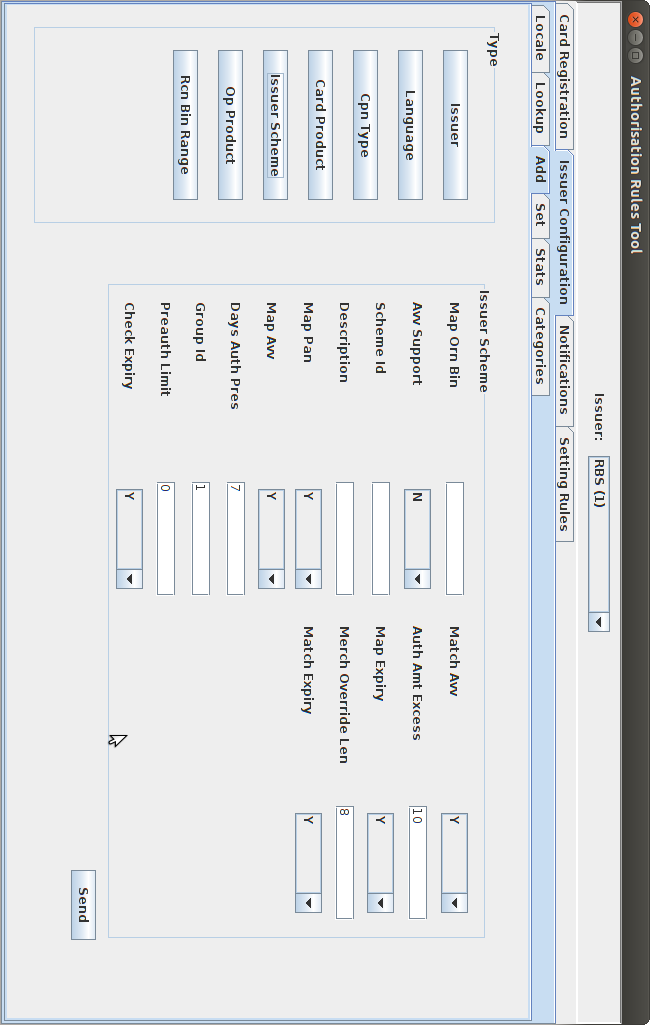
\includegraphics[width=\textwidth]{smart_generated_ui.png}



\todo{Reflect on using oil they way it was intended without instruction}

\subsubsection{Maintenance}


\subsection{Testing}





Because Cronos was just another generic server component it was assumed that interfacing SMART with it would be relatively straightforward. The communication code for the Retail API Server had been used in SMART for years. To isolate the Cronos specific code, several sub packages were created within SMARTs MVC structure. \cite{Something about reusablity through modularity}


\subsection{Maintenance}
SMART is window into platform, lots of errors not my fault

\subsection{OIL}
\label{OIL}
Orbiscom Interface Language is an in house Interface Definition Language. It is used to specify how various components communicate with each other. It can be used to specify basic data objects, request definitions and their behavior. I used OIL extensively throughout the internship. There was some existing documentation that was helpful, but the bulk to the knowledge I acquired was from asking questions and reading the OIL grammar file. The OIL grammar file is a standard Backus–Naur Form grammar and was quite easy to read because BNF grammars were covered extensively in the Discrete Mathematics and Compiler Design courses taken in second and third year respectively. There were some difficulties surrounding the implementation of the OIL compiler. Functionality described in the grammar was not implemented in the compiler. The most prominent being the inability to set default values for request parameters. \todo{Draw more attention to the fact I found this?}
OIL is a fully fledged language with its own compiler. The compiler generates program code \todo{How is not just a code generator?} that can then be compiled. At the moment, Java and Flex \todo{Correct?} can be generated using OIL.
OIL is used throughout the InControl Platform. Virtualy every component uses it in some respect. Even the components that do not use OIL directly, e.g. do not call the OIL generated code, use OIL indirectly as all of the XML messages are generated by OIL classes.
During my time at MasterCard I too used OIL extensively. If a new request is needed it must be created using OIL. There are several steps involved, beginning with creating the database code to service the request. The stored database procedure is invoked by and OIL request handler. This handler must be written manually. I wrote a script to automate this process somewhat. The handler is invoked by an OIL generated handler, which is configured to run when a specific request comes in. This request is again an OIL generated type. The steps to add a new request to a component called Cronos follows
\subsubsection{Create the stored procedure}
A stored procedure is set of pre-compiled SQL statements stored inside a database. This example is just a simple select statement but any SQL is valid. Stored procedures are saved to \textit{release}/database/procedures/src/o\_\textit{module}.pls, e.g. \textbf{\textit{r12q4/database/procedures/src/o\_cronos.pls}}. \todo{Does that look a bit much}Each stored procedure package consists of two sections, procedure prototype definitions and procedure bodies. This is the same as any programming language, the prototypes are function heads and the implementing code is contained within the body.
A definition:
\begin{verbatim}
PROCEDURE GetIssuerConfig (
        p_issuer_id IN VARCHAR2,
        r_issuer_config OUT Globals.ref_cursor);
\end{verbatim}
Here the procedure takes a string and a reference cursor. A cursor acts like a pointer to the result set returned by the query. A ref cursor is similar, the key difference being that it is not bound to a single result set and can also be passed back up to the client, which is somewhat important. If no result set is returned, ie, an insert, no ref cursor is need.
The implementing code. This is just standard SQL code
\begin{verbatim}
PROCEDURE GetIssuerConfig (
        p_issuer_id IN VARCHAR2,
        r_issuer_config OUT Globals.ref_cursor)
    IS
    BEGIN
        OPEN r_issuer_config FOR
            SELECT issuer_name, authentication_type, authorisation_type, session_timeout,
            authenticate_pan_password, allow_change_email_addr, allow_set_user_name, create_date, update_date
            FROM issuer_config
            WHERE issuer_id = p_issuer_id;
    END;
\end{verbatim}
The stored procedure must then be loaded into the database. If there are any errors in the stored procedure file loading will fail and the entire file and all of the contained procedure will be rejected. It is generally a good idea to test the procedure works as intended before writing code to access it. It can be executed by specifying the package and procedure name. If the procedure requires a reference cursor it must also be declared
\begin{verbatim}
var blah refcursor
execute 'cronos12q4db.GetIssuerConfig('1', :blah);
\end{verbatim}

\subsubsection{OIL Interface}
There are two files used to define the classes OIL generates, the OIL definition file and the OIL procedure definition file. The procedure definition file is nearly identical to the stored procedure definition file, so it may be easier to write it first and then the definition file.

The OIL definition file, e.g. \textbf{\textit{cronos.oil}} is used to define the request and any data types needed by that request. The file begins with an interface definition, this is the package where the generated code is stored. This is optionally followed by any imports needed. This allows OIL files to be split up very easily. Typically, that is, by convention only, data types are defined. The two built in data types are \textbf{String} and \textbf{Number}. Any user defined data types are collections of these and other used defined data types. Default values are supported. This is where the default values mentioned in the Retail API Server section come from. They are specified in the OIL files and are thus hard coded into the generated Java code.
\begin{verbatim}
 type IssuerConfig
    {
        String IssuerName;
        Number AuthenticationType;
        String AuthorisationType;
        Number SessionTimeout;
        String AuthenticatePanPassword;
        String AllowChangeEmailAddr;
        String AllowSetUserName = "N";
    }
\end{verbatim}
The request definitions follow the type definitions
\begin{verbatim}
request GetIssuerConfig(
        required String IssuerId)
    {
        response
        {
            IssuerConfig IssuerConfig;
        }
    }
\end{verbatim}
This is a very basic example of what OIL is capable of and will result in a basic data model Object and request definition. OIL supports annotations to support various features, such as comments to be included in the generated code and enforcing mandatory members in request parameters etc. Arrays are also supported. They can be restricted to containing elements of a specified type or multiple elements of different specified types. OIL definition files also have access to a Context Object. Values can be stored and retrieved from this Object when the generated code is running. This is particularly useful for large and complex operations. Values can be saved in the context to avoid having to pass them between requests.

The OIL procedure file maps the values returned by the stored procedure to the members of the OIL Object returned in the query response. It is an Object relational mapping similar to technologies like Hibernate \todo{Might be stretching it a bit there}
\begin{verbatim}
 procedure GetIssuerConfig[Cronos12q4DB.GetIssuerConfig] (
        String IssuerId => p_issuer_id)
    {
        output
        {
            IssuerConfig IssuerConfig <= r_issuer_config
            {
                String IssuerName <= issuer_name;
                Number AuthenticationType <= authentication_type;
                String AuthorisationType <= authorisation_type;
                Number SessionTimeout <= session_timeout;
                String AuthenticatePanPassword <= authenticate_pan_password;
                String AllowChangeEmailAddr <= allow_change_email_addr;
                String AllowSetUserName <= allow_set_user_name;
            }
        }
    } 
\end{verbatim}
One important thing to note here is that the type definitions declared in the OIL definition file must be imported into the OIL procedures file. Another more subtle issue is the presence of duplicate column names in a result set. The values will always be taken from the first column in the result set. The easiest way I found to fix this was to modify the stored procedure to rename the conflicting columns in the result set. Oracle makes this very easy, the column name need only be appended with the desired name, i.e. \textit{ table\_name.column\_name "desired\_name" }

The OIL compiler is then ran against the files which outputs several classes per request.  The final step is to write a handler. The handler is executed by the server on receiving a particular request, mapped in the config files as outlined on page \pageref{handlerset}

\subsection{OIL Handler}
An appropriate handler class must be created in order to service the request. The handler must implement OilProcessor, specifically the OIL processor generated above \todo{Hierarchy tree here}. The purpose of the second, generated processor is to enforce parameter types. \todo{Get input}. For simple queries very little is needed. The request parameters are extracted form the incoming request object. The stored procedure is then called with these parameters. The output is put into the response object and sent back to the calling client.

\begin{verbatim}
package com.orbiscom.cronos.oil;

import java.sql.Connection;

import com.orbiscom.apollo.core.MessageProcessingException;
import com.orbiscom.atlas.core.ErrorMessage;
import com.orbiscom.atlas.core.MessageContext;
import com.orbiscom.atlas.xml.ApplicationHandler;
import com.orbiscom.cronos.oil.proc.GetIssuerListOutput;
import com.orbiscom.cronos.oil.proc.GetIssuerListProc;
import com.orbiscom.oil.db.ProcFactory;
import com.orbiscom.oil.db.StoredProcedureException;


public class GetIssuerListHandler
	implements GetIssuerListProcessor
{
	private final GetIssuerListProc iProc;

	public GetIssuerListHandler()
		throws StoredProcedureException
	{
		iProc = ProcFactory.getProc(GetIssuerListProc.class);
	}

	public void process(MessageContext ctx, GetIssuerListRequest request, GetIssuerListResponse response)
		throws MessageProcessingException
	{
		try
		{
			Connection conn = ctx.getIssuerDatabaseConnection(ApplicationHandler.APPLICATION_DB);

			GetIssuerListOutput out = iProc.call(ctx, conn);

			response.setIssuers(out.getIssuers());
		}
		catch (MessageProcessingException ex)
		{
			throw ex;
		}
		catch (Exception ex)
		{
			throw new ErrorMessage.GeneralError(ex);
		}
	}
}
\end{verbatim}
Writing these handler is particularly tedious. However, as they are usually very similar the process can, and was, automated with a simple script.
The handler must then be added to the servers handler configuration file as shown on page \pageref{handlerset}

\cite{Stored procedure for dummys}
\cite{http://wiki.orbiscom.com/index.php/OIL}

\section{Web Admin Console}
Objectives. Describe Web Admin Console. Describe what was done (BUGS!). How were bugs tested / found?. Don't forget the impacted work on Cronos.
\section{Conclusion}
Technical Conclusion. Goals. BCS goals.
\section{References}

\section{Appendices}


\end{document}
